In questa sezione sono illustrate la metodologia di test, le metriche utilizzate e risultati ottenuti dai test svolti.\\
Nella sezione \autoref{sec:test_intro} sono illustrati gli obiettivi dei test e la metodologia con la quale sono svolti. Nella \autoref{sec:test_metriche} sono descritte le metriche usate per svolgere i test. Nella \autoref{sec:test_risultati} sono riportati i risultati ottenuti dai test.

\section{Introduzione}
\label{sec:test_intro}
La metodologia di test adottata ha lo scopo di valutare automaticamente e in modo ripetibile le prestazioni del sistema di correzione. Tale metodologia è utile durante lo sviluppo del sistema di correzione, in quanto rende possibile quantificare l'impatto delle modifiche apportate al funzionamento e alla configurazione.\\
Inoltre, i test svolti in questo capitolo rendono possibile:
\begin{itemize}
\item Valutare le performance del sistema su vari tipi e intensità di errore. Come illustrato nel \autoref{sec:dataset}, per ogni frase perturbata nel dataset, sono presenti 9 versioni perturbate con diverse superpipeline. Valutando le performance di correzione sulle diverse tipologie di frasi, è possibile determinare come si comporta il sistema di correzioni di fronte a diversi tipi di errore.

\item Confrontare le performance del sistema di correzione su diverse versioni del dataset. Nel \autoref{sec:dataset} sono infatti state definite due versioni del dataset, \dsta\ e \dstb, che differiscono per la lunghezza delle frasi. Portare a termine i test su entrambe le versioni permette quindi di capire quanto la lunghezza delle frasi influisca sulle prestazioni del sistema di correzione.

\item Confrontare il sistema di correzione sviluppato con altri sistemi di OCR post-processing per avere un riscontro con il quale meglio valutare i risultati ottenuti. A tale scopo, si utilizza come confronto la metodologia di correzione proposta in \cite{hamalainen2019paft}, già illustrata nella \autoref{sec:arte_nmt}; l'approccio utilizzato è però leggermente modificato, e utilizza una combinazione di FastText e Word2Vec per trovare le parole semanticamente simili a quelle errate (a differenza del solo Word2Vec come nel paper originale). Per distinguere il metodo sviluppato da quello usato come confronto, si ci riferirà con:
	\begin{itemize}
	\item \textbf{Bert} al metodo sviluppato e oggetto di questa tesi.
	\item \textbf{Ftwv} al metodo appena descritto usato come confronto.
	\end{itemize}

\end{itemize}

\paragraph{Metodologia} Sono dati:
\begin{itemize}
\item L'insieme $D = \{\textit{\dsta}, \textit{\dstb} \}$ dei dataset
\item L'insieme $M = \{\textit{Bert}, \textit{Ftwv}\}$ dei metodi di correzione
\end{itemize}
Ogni frase $f$ in \dsta\ o \dstb contiene il testo originale (\textit{text}), e le sue versioni perturbate nel campo \textit{perturbed}. Dato il metodo $m \in M$ che si vuole valutare, e data una delle versioni perturbate $v$ della frase nel campo \textit{perturbed}, si produce la tripla in \autoref{tab:test_tripla}.

\begin{table}[H]
\centering
\begin{tabular}{cc}
\textbf{Nome Campo} & \textbf{Descrizione} \\
\hline
$t_{or}$ & Testo originale (\textit{text)}\\
$t_{pe}$ & Testo perturbato ($v$)\\
$t_{co}$ & $v$ corretta con il metodo $m$
\end{tabular}
\caption{Tripla contenente la frase corretta con uno dei metodi in $M$}
\label{tab:test_tripla}
\end{table}
\noindent
Dato un dataset $d \in D$, si producono 9 di queste triple per ogni frase $f \in d$, una per ognuna delle versioni perturbate presenti nel campo \textit{perturbed} di  $f$. Le triple sono raggruppate in 9 insiemi (T1, T2, T3, S1, S2, S3, M1, M2, M3) in base alla superpipeline di riferimento del campo $t_{pe}$. Su ognuno di questi insiemi è quindi possibile calcolare le metriche illustrate nella \autoref{sec:test_metriche}.

\section{Metriche}
\label{sec:test_metriche}
La valutazione della correzione avviene attraverso le metriche definite in questa sezione. Le metriche definite sono:
\begin{enumerate}
\item Errori corretti per errore presente ($C/P$).
\item Errori introdotti per carattere ($In/Ch$).
\item Errori introdotti per errore corretto ($I/C$).
\item Riduzione nella distanza di Levenshtein. ($LDR$).
\item Distanza di Levenshtein totale ($LDT$).
\end{enumerate}
\noindent
Prima di spiegare nel dettaglio le metriche introdotte, è spiegato il concetto di "errore delimitato" usato nelle prime tre metriche.

\paragraph{Errore delimitato} Siano date:
\begin{itemize}
\item $s$: una sequenza di testo considerata corretta.
\item $s\prime$: una sequenza di testo che differisce da $s$ per alcuni errori. 
\end{itemize}
Si definiscono "\textit{matching block}" tutte le sottosequenze coincidenti di $s$ e $s\prime$, attraverso le quali è anche possibile allineare le due sequenze. Si prendano ad esempio le sequenze \textit{"Adesso io preferisco"} e\textit{"Addcso io prioferisco"}; è possibile allinearne i matching block come segue:
\begin{center}
\noindent
\texttt{\underline{Ad} es \underline{so io pr} e\ \ \underline{ferisco}}\\
\texttt{\underline{Ad} dc \underline{so io pr} io \underline{ferisco}}
\end{center}
Si noti come i matching block siano stati sottolineati. Le sottosequenze che non sono comprese nei matching block, nella seconda frase dell'esempio \textit{"dc"} e \textit{"io"}, sono quelle che contengono le differenze fra le due frasi, che in questo caso corrispondono agli errori. Queste sottosequenze sono chiamate \textit{errori delimitati}.\\
Si prenda ad esempio la frase:
\begin{center}
\textit{"Adesso io preferisco parlare spontaneamente."}
\end{center}
In \autoref{tab:test_erroridel} sono date alcune versioni perturbate della stessa frase. Gli errori delimitati sono segnati fra parentesi quadre:

\begin{table}[H]
\centering
\begin{tabular}{cc}
\textbf{Esempio} & \textbf{Errori delimitati}\\
\hline
A[,]des[,]so io preferisco parlare spontaneamente. & 2 \\
Ad[dc]so io pr[io]ferisco parlare spontaneamente. & 2 \\
Ad[c]sso[.] io pr[c]f[c]risc parlare spontaneamente. & 3\\
\end{tabular}
\caption{Versioni perturbate della frase di esempio con gli errori delimitati segnati dalle parentesi quadre}
\label{tab:test_erroridel}
\end{table}
\noindent
Si noti come ogni errore delimitato contribuisca al conteggio del numeri di errori con un +1 indipendentemente dal numero di caratteri da cui è composto.

Data quindi una qualsiasi tripla $t$ appartenente a uno dei 9 insieme definiti in precedenza, e formata dai campi $t_{or}$, $t_{pe}$, $t_{co}$, sono date le seguenti definizioni:

\begin{itemize}
\item \textbf{Errori corretti:} numero di errori delimitati che sono in $t_{pe}$ ma non in $t_{co}$. Più informalmente, è il numero di errori che il sistema di correzione utilizzato è riuscito a correggere.
\item \textbf{Errori presenti:} numero di errori delimitati che sono in $t_{pe}$. Più informalmente, è il numero di errori che la superpipeline di perturbazione utilizzata ha generato in $t_{pe}$.
\item \textbf{Errori introdotti:} numero di errori delimitati in $t_{co}$ che non sono né in $t_{pe}$, né in $t_{or}$. Più informalmente, è il numero di errori che il sistema di correzione ha introdotto provando a correggere $t_{pe}$.
\end{itemize}

Data quindi una qualsiasi tripla $t$ appartenente a uno dei 9 insieme definiti in precedenza, sono definite le seguenti funzioni:
\begin{itemize}
\item $f_{co}(t)$: data una tripla $t$, ne restituisce il numero di errori corretti.
\item $f_{pr}(t)$: data una tripla $t$, ne restituisce il numero di errori presenti.
\item $f_{in}(t)$: data una tripla $t$, ne restituisce il numero di errori introdotti.
\end{itemize}
\noindent
Date queste definizioni, sono di seguito definite le metriche elencate in precedenza.


\paragraph{Errori corretti per errore presente ($C/P$)} Lo scopo di questa metrica è quello di calcolare la percentuale di errori che il sistema di correzione riesce a risolvere. Dato un insieme $I$ di triple $(\text{$t_{or}$, $t_{pe}$, $t_{co}$})$, è possibile definire $C/P$ come segue:
\begin{equation}
C/P = \frac{
    \sum_{t \in I} f_{co}(t)
}{
	\sum_{t \in I} f_{pr}(t)
}
\end{equation}
$C/P$ vale 0 se il sistema di correzione non corregge alcun errore, mentre vale 1 se il sistema di correzione li corregge tutti. \E\ quindi chiaro come più alto è il valore di $C/P$, migliori sono le performance di correzione.


\paragraph{Errori introdotti per frase ($In/Ch$)} Lo scopo di questa metrica è quello di quantificare gli errori che il sistema di correzione introduce. Dato un insieme $I$ di triple $(\text{$t_{or}$, $t_{pe}$, $t_{co}$})$, è possibile definire $In/Ch$ come segue:
\begin{equation}
In/Ch = \frac{
    \sum_{t \in I} f_{in}(t)
}{
	|I|
}
\end{equation}
La metrica è divisa per il numero caratteri nel dataset, in modo tale da permettere anche la comparazione fra dataset con lunghezze differenti. In questo caso, valori più bassi di $In/Ch$ sono desiderabili, in quanto si vuole evitare che il sistema di correzione non introduca nuovi errori.

\paragraph{Errori introdotti per ogni errore corretto ($I/C$)} Lo scopo di questa metrica è quello di misurare il rapporto fra gli errori che il sistema di correzione introduce durante la correzione, e gli errori presenti che invece vengono corretti. Dato un insieme $I$ di triple $(\text{$t_{or}$, $t_{pe}$, $t_{co}$})$, è possibile definire $I/C$ come segue:
\begin{equation}
I/C = \frac{
    \sum_{t \in I} f_{in}(t)
}{
	\sum_{t \in I} f_{co}(t)
}
\end{equation}
In questo caso, a valori più bassi di $I/C$ corrispondono performance migliori del sistema di correzione. Più precisamente:
\begin{itemize}
\item Se $I/C \geq 1$, significa che il sistema di correzione sta introducendo più errori di quanti ne corregge, peggiorando nel complesso il testo in input.

\item Se $0 < I/C < 1$, significa che il sistema di correzione sta correggendo più errori di quanti ne introduce, migliorando quindi il testo in input. Più il valore di $I/C$ approssima lo 0, migliori sono le performance di correzione.
\end{itemize}

\paragraph{Riduzione nella distanza di Levenshtein ($LDR$)}
Lo scopo di questa metrica è quello di misurare quanto il processo di correzione avvicina la frase perturbata a quella originale. Si misura quindi la differenza in distanza di Levenshtein fra frase originale e frase perturbata e fra frase originale e frase corretta. Lo scarto fra queste distanze indica la riduzione in distanza. Dato un insieme $I$ di triple $(\text{$t_{or}$, $t_{pe}$, $t_{co}$})$, è possibile definire $LDR$ come segue:
\begin{equation}
LDR = \frac{
\sum_{t \in I}d(t_{or},t_{pe}) - d(t_{or},t_{co})}{\sum_{t \in I}|t_{or}|}
\end{equation}
Il valore ottenuto è diviso per la somma dei caratteri totali contenuti nell'insieme I. In questo modo la differenza è espressa nel rapporto riduzione su numero di caratteri, consentendo così di confrontare misurazioni su dataset differenti. Per questa metrica valori maggiori indicano migliori performance del sistema di correzione.


\paragraph{Distanza di Levenshtein totale ($LDT$)}
Lo scopo di questa metrica è quello di misurare la distanza totale fra le frasi originali e quelle corrette. Dato un insieme $I$ di triple $(\text{$t_{or}$, $t_{pe}$, $t_{co}$})$, è possibile definire $LDT$ come segue:
\begin{equation}
LDT = \frac{
\sum_{t \in I}d(t_{or},t_{co})}{\sum_{t \in I}|t_{or}|}
\end{equation}
Il valore ottenuto è diviso per la somma dei caratteri totali contenuti nell'insieme I. In questo modo la differenza è espressa nel rapporto riduzione su numero di caratteri, consentendo così di confrontare misurazioni su dataset differenti. Per questa metrica valori più bassi indicano migliori performance del sistema di correzione.


\section{Risultati}
\label{sec:test_risultati}

Lo scopo dei test in questa sezione è quello di valutare le performance del sistema di correzione sviluppato e confrontarle a quelle del sistema Ftwv. Si vuole inoltre misurare l'impatto della lunghezza della frasi da correggere sulle performance di correzione. Per fare ciò, si eseguiranno i test sulle seguenti configurazioni:
\begin{itemize}
\item \textbf{Bert@50}: sistema di correzione Bert con dataset \dsta.
\item \textbf{Bert@100}: sistema di correzione Bert con dataset \dstb.
\item \textbf{Ftwv@50}: sistema di correzione Ftwv con dataset \dsta.
\item \textbf{Ftwv@100}: sistema di correzione Ftwv con dataset \dstb.
\end{itemize}





\paragraph{Errori corretti per errore presente ($C/P$)}
In \autoref{fig:test_res_cp_gra} e \autoref{fig:test_res_cp} sono riportate le misurazioni per la metrica $C/P$. Dati i risultati, è possibile fare le seguenti osservazioni:
\begin{itemize}
\item Per ogni superpipeline, le configurazioni che usano frasi più lunghe ottengono risultati migliori rispetto alle controparti che utilizzano frasi da 50 caratteri. Questo fatto supporta l'ipotesi che la presenza di contesto più amplio attorno a un errore possa aiutare durante la correzione.

\item Il sistema di correzione sviluppato ottiene performance significativamente maggiori nelle token superpipeline. Questo era il risultato atteso, in quanto la correzione dei word error è stato il focus principale durante lo sviluppo del sistema.

\end{itemize}

\begin{table}[H]
\centering
\begin{tabular}{c|cc|cc}
\textbf{Superpipeline} & \textbf{Bert@50} &  \textbf{Ftwv@50} & \textbf{Bert@100} & \textbf{Ftwv@100}\\
\hline
M1& 0.29& 0.17& 0.32& 0.22\\
M2& 0.28& 0.18& 0.33& 0.25\\
M3& 0.23& 0.16& 0.26& 0.24\\
S1& 0.26& 0.14& 0.27& 0.15\\
S2& 0.25& 0.17& 0.25& 0.17\\
S3& 0.27& 0.16& 0.28& 0.16\\
T1& 0.33& 0.16& 0.4& 0.24\\
T2& 0.34& 0.18& 0.4& 0.27\\
T3& 0.29& 0.17& 0.37& 0.28\\
\end{tabular}
\caption{Misurazioni di $C/P$ su tutti gli insiemi di frasi}
\label{fig:test_res_cp_gra}
\end{table}

\begin{figure}[H]
\centering
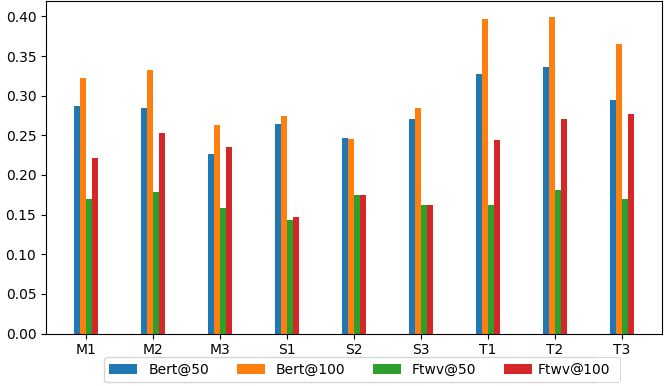
\includegraphics[width=\textwidth]{immagini/test/cp}
\caption{Misurazioni di $C/P$ su tutti gli insiemi di frasi}
\label{fig:test_res_cp}
\end{figure}

\paragraph{Errori introdotti per carattere ($In/Ch$)}
In \autoref{fig:test_res_if_gra} e \autoref{fig:test_res_if} sono riportate le misurazioni per la metrica $In/Ch$. Dati i risultati si possono fare le seguenti osservazioni:
\begin{itemize}
\item In questo caso la lunghezza delle frasi non influenza i risultati ottenuti, che sono comparabili a parità di sistema di perturbazione.

\item Si nota un amplio scarto fra i due sistemi di correzione: ciò in parte è attribuibile all'efficacia dello stadio di validazione durante la correzione nel sistema Bert. Non è però possibile escludere che il sistema Ftwv sia particolarmente prono all'introduzione di errori durante la correzione.
\end{itemize}

\begin{table}[H]
\centering
\begin{tabular}{c|cc|cc}
\textbf{Superpipeline} & \textbf{Bert@50} &  \textbf{Ftwv@50} & \textbf{Bert@100} & \textbf{Ftwv@100}\\
\hline
M1& 0.0051& 0.0226& 0.0055& 0.0245\\
M2& 0.0056& 0.0217& 0.0055& 0.0235\\
M3& 0.0063& 0.0206& 0.0076& 0.024\\
S1& 0.0044& 0.024& 0.0042& 0.0236\\
S2& 0.0043& 0.0235& 0.0042& 0.023\\
S3& 0.0043& 0.0219& 0.0046& 0.0212\\
T1& 0.0049& 0.0238& 0.0048& 0.0255\\
T2& 0.0051& 0.0232& 0.005& 0.0253\\
T3& 0.0058& 0.023& 0.0056& 0.0259\\
\end{tabular}
\caption{Misurazioni di $In/Ch$ su tutti gli insiemi di frasi}
\label{fig:test_res_if_gra}
\end{table}

\begin{figure}[H]
\centering
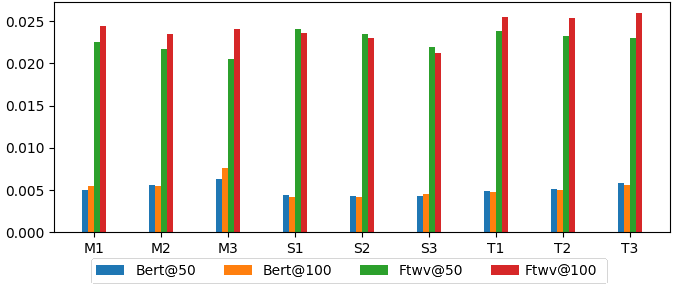
\includegraphics[width=\textwidth]{immagini/test/if}
\caption{Misurazioni di $In/Ch$ su tutti gli insiemi di frasi}
\label{fig:test_res_if}
\end{figure}

\paragraph{Errori introdotti per errore corretto ($I/C$)}
In \autoref{fig:test_res_ic_gra} e \autoref{fig:test_res_ic} sono riportate le misurazioni per la metrica $I/C$. Dati i risultati si possono fare le seguenti osservazioni:
\begin{itemize}
\item Sono confermate le osservazioni fatte in precedenza: il sistema Bert corregge più errori e ne introduce di meno al sistema Ftwv. Con la sola eccezione di S1, il sistema bert ha un $I/C$ ampiamente inferiore a 1 su tutte le superpipeline e su entrambe le lunghezze di frasi. Ciò implica che il sistema corregge più errori di quanti ne introduce.

\item Per questa metrica è presente una lieve ma non trascurabile differenza di prestazioni derivante dalla lunghezza delle frasi: frasi più lunghe, anche in questo caso, portano a risultati migliori.
\end{itemize}

\begin{table}[H]
\centering
\begin{tabular}{c|cc|cc}
\textbf{Superpipeline} & \textbf{Bert@50} &  \textbf{Ftwv@50} & \textbf{Bert@100} & \textbf{Ftwv@100}\\
\hline
M1& 0.36& 2.79& 0.35& 2.3\\
M2& 0.32& 2.01& 0.26& 1.49\\
M3& 0.29& 1.37& 0.3& 1.05\\
S1& 1.02& 10.26& 0.91& 9.38\\
S2& 0.89& 6.75& 0.83& 6.4\\
S3& 0.45& 3.76& 0.44& 3.53\\
T1& 0.4& 3.98& 0.32& 2.8\\
T2& 0.32& 2.74& 0.26& 1.96\\
T3& 0.28& 1.97& 0.22& 1.36\\
\end{tabular}
\caption{Misurazioni di $I/C$ su tutti gli insiemi di frasi}
\label{fig:test_res_ic_gra}
\end{table}

\begin{figure}[H]
\centering
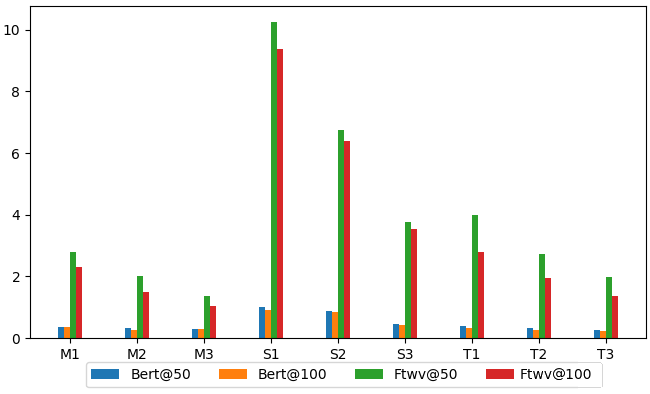
\includegraphics[width=\textwidth]{immagini/test/ic}
\caption{Misurazioni di $I/C$ su tutti gli insiemi di frasi}
\label{fig:test_res_ic}
\end{figure}


\paragraph{Riduzione nella distanza di Levenshtein ($LDR$)}
In \autoref{fig:test_res_ldr_gra} e \autoref{fig:test_res_ldr} sono riportate le misurazioni per la metrica $LDR$. Dati i risultati si possono fare le seguenti osservazioni:

\begin{itemize}
\item \E\ possibile confermare quanto visto precedenza: il sistema Bert corregge un maggior numero di errori e ne introduce di meno rispetto al sistema Ftwv. Ciò si traduce in una riduzione positiva della distanza di Levenshtein.
\item Anche in questo caso è presente un delta rilevante fra la prestazioni di entrambi i sistemi con frasi di lunghezza diversa. In questo caso, però, la differenza è più marcata nei risultati del sistema bert.

\item Il sistema Bert presenta una riduzione negativa sulle pipeline S1 e S2, mentre la riduzione positiva è quasi nulla nella pipeline S3. Questo conferma quanto già osservato, ovvero che il sistema di correzione sviluppato non corregge in modo ottimale i word segmentation error. 
\end{itemize}
\vfill
\newpage

\begin{table}[H]
\centering
\begin{tabular}{c|cc|cc}
\textbf{Superpipeline} & \textbf{Bert@50} &  \textbf{Ftwv@50} & \textbf{Bert@100} & \textbf{Ftwv@100}\\
\hline
M1& 0.01& -0.04& 0.01& -0.04\\
M2& 0.01& -0.04& 0.02& -0.03\\
M3& 0.02& -0.03& 0.03& -0.02\\
S1& -0.0& -0.05& -0.0& -0.05\\
S2& -0.0& -0.04& -0.0& -0.04\\
S3& 0.0& -0.04& 0.0& -0.04\\
T1& 0.01& -0.05& 0.01& -0.05\\
T2& 0.01& -0.04& 0.02& -0.04\\
T3& 0.02& -0.04& 0.02& -0.04\\
\end{tabular}
\caption{Misurazioni di $LDR$ su tutti gli insiemi di frasi}
\label{fig:test_res_ldr_gra}
\end{table}

\begin{figure}[H]
\centering
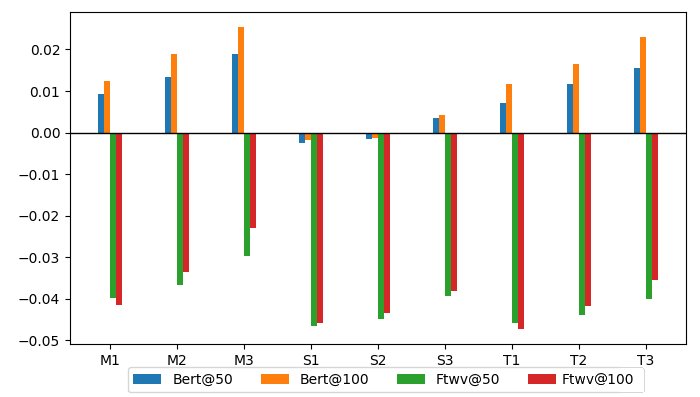
\includegraphics[width=\textwidth]{immagini/test/ldr}
\caption{Misurazioni di $LDR$ su tutti gli insiemi di frasi}
\label{fig:test_res_ldr}
\end{figure}
\vfill

\paragraph{Distanza di Levenshtein totale ($LDT$)}
In \autoref{fig:test_res_ldt_gra} e \autoref{fig:test_res_ldt} sono riportate le misurazioni per la metrica $LDT$. I risultati ottenuti confermano le osservazioni riportate in precedenza.

\begin{table}[H]
\centering
\begin{tabular}{c|cc|cc}
\textbf{Superpipeline} & \textbf{Bert@50} &  \textbf{Ftwv@50} & \textbf{Bert@100} & \textbf{Ftwv@100}\\
\hline
M1& 0.06& 0.1& 0.05& 0.11\\
M2& 0.07& 0.12& 0.07& 0.12\\
M3& 0.12& 0.16& 0.11& 0.16\\
S1& 0.02& 0.06& 0.02& 0.06\\
S2& 0.02& 0.07& 0.02& 0.07\\
S3& 0.04& 0.08& 0.04& 0.08\\
T1& 0.04& 0.1& 0.04& 0.1\\
T2& 0.05& 0.11& 0.05& 0.11\\
T3& 0.08& 0.13& 0.07& 0.13\\
\end{tabular}
\caption{Misurazioni di $LDT$ su tutti gli insiemi di frasi}
\label{fig:test_res_ldt_gra}
\end{table}

\begin{figure}[H]
\centering
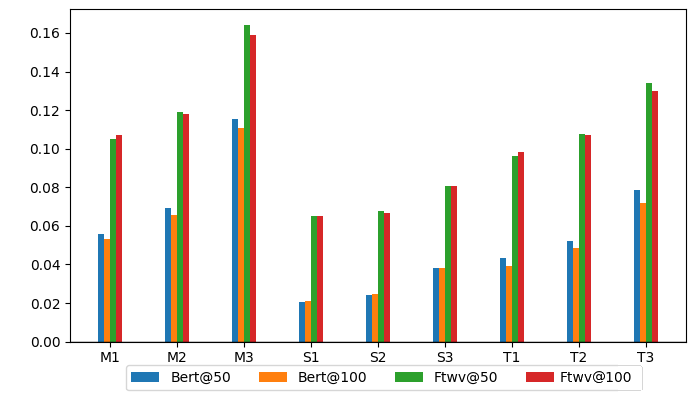
\includegraphics[width=\textwidth]{immagini/test/ldt}
\caption{Misurazioni di $LDT$ su tutti gli insiemi di frasi}
\label{fig:test_res_ldt}
\end{figure}

\newpage

\paragraph{Conclusioni}
Dai risultati ottenuti in questa sezione è possibile trarre le seguenti conclusioni:
\begin{itemize}
\item Il sistema Bert ottiene performance migliori rispetto al sistema Ftwv per ogni singola metrica. I risultati mostrano come il sistema Bert corregga più errori rispetto al sistema Ftwv. La differenza più marcata risiede però nell'introduzione di nuovi errori, ambito nel quale il sistema Bert ha prestazioni decisamente migliori.

\item Una lunghezza maggiore della frase da correggere è correlata ad un aumento delle performance di correzione. Ciò è imputabile al funzionamento dei sistemi di correzione testati, che usano il contesto intorno ad un errore per effettuare la correzione. Più ampio è il contesto, migliori sono i risultati.

\item Il sistema Bert ottiene scarsi risultati sulle superpipeline di segmentazione. Ciò è dovuto principalmente al fatto che la correzione è più focalizzata sui word error. La correzione e l'individuazione degli errori di segmentazione, inoltre, è un problema complicato e diverso dalla correzione dei word error: è quindi necessario sviluppare un sistema che riesca ad individuare e correggere più tipi di errori di segmentazione in modo più comprensivo.
\end{itemize}

